\documentclass[twoside,a4paper,openright,titlepage,draft]{ctexrep}
\usepackage[final]{graphicx}
\usepackage{subfig}
% \usepackage{subcaption}
\usepackage{extarrows}
\usepackage{multicol}
\usepackage{float}
\usepackage{amsmath}
\usepackage{subfig}
\usepackage{cancel}
\usepackage{wrapfig}
\graphicspath{{./pictures}}
\setcounter{secnumdepth}{3}

\begin{document}
\section{简单差动对}
\begin{multicols}{2}
    \begin{figure}[H]
        \centering
        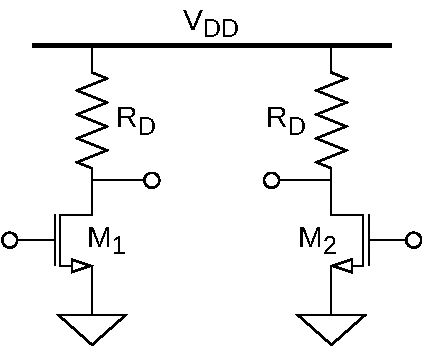
\includegraphics[width=0.8\columnwidth]{simpledifferentialpair.drawio.pdf}
        \caption{简单差动对}
        \label{fig:简单差动对}
    \end{figure}
    \columnbreak
    \paragraph{缺点}
    输入$V_{in}$会引起电流$I_D$的变化,导致增益改变。\\
    所以基本不可以使用,因为增益一直在变导致波形失真。
\end{multicols}
\section{差动对}
\begin{multicols}{2}
    \begin{figure}[H]
        \centering
        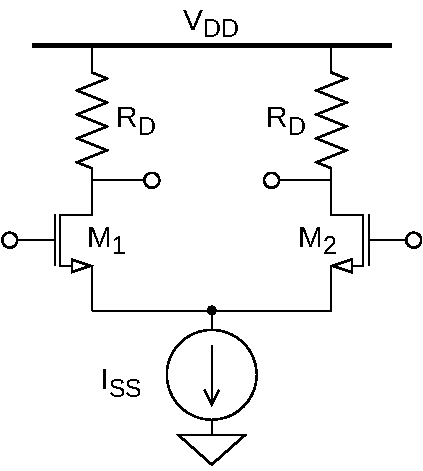
\includegraphics[width=0.8\columnwidth]{differentialpair.drawio.pdf}
        \caption{差动对}
        \label{fig:差动对}
    \end{figure}
    \columnbreak
    \begin{equation}
        I_{d1} = I_{d2} = \frac{I_{ss}}{2}
    \end{equation}
    当$V_{in1/2} = 1V$与$V_{in1/2} = 2V$的时候都没区别。
    \subsection{大信号分析}
    寻找线性放大区间
\end{multicols}
\begin{align}
    &\begin{cases}
        I_{D1} &= \frac{1}{2}\mu_nC_{ox}(\frac{W}{L})(V_{in}^+ - V_{TH1})^2 \\
        I_{D2} &= \frac{1}{2}\mu_nC_{ox}(\frac{W}{L})(V_{in}^- - V_{TH2})^2 \\
    \end{cases}\\
    &V_{in1} - V_{in2} = \sqrt{\frac{2I_{D1}}{\mu_nC_{ox}\frac{W}{L}}} - \sqrt{\frac{2I_{D2}}{\mu_nC_{ox}\frac{W}{L}}}\\
    &(V_{in1} - V_{in2})^2 = \frac{2}{\mu_nC_{ox}\frac{W}{L}}(I_{SS} - 2\sqrt{I_{D1}I_{D2}})
\end{align}
\subsection{小信号分析}
\subsubsection{Gain}
\begin{figure}[H]
    \centering
    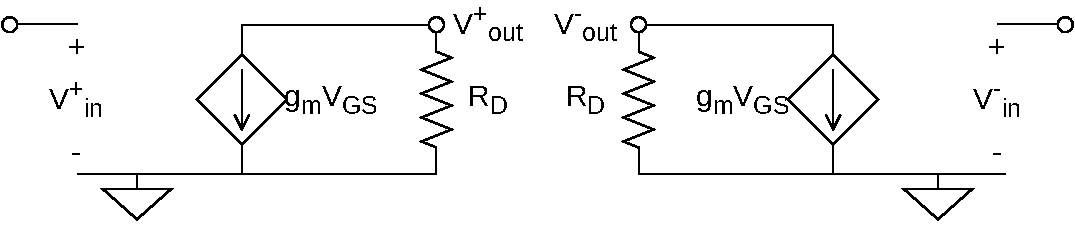
\includegraphics[width=0.9\textwidth]{smallsignaldiff.drawio.pdf}
    \caption{小信号模型图}
    \label{fig:smallsignal}
\end{figure}
\begin{align}
    &\begin{cases}
        V_{out}^+ &= -g_mV_{in}^+ \\
        V_{out}^- &= -g_mV_{in}^-
    \end{cases} \\
    V_{out} &= (V_{out}^+ - V_{out}^-)\notag\\
    &= g_m(V_{in}^+ - V_{in}^-)R_D\notag\\
    &= -g_mV_{in}R_D \\
    A_V &= \frac{V_{out}}{V_{in}} = -g_mR_D
\end{align}
\end{document}